\documentclass[11pt]{article}

\usepackage[margin=1in]{geometry}
\setlength{\headheight}{13.6pt}
\usepackage{fancyhdr}
\pagestyle{fancy}
\usepackage{scalerel}
\usepackage{mathtools}
\usepackage{amssymb}
\usepackage{xparse}
\usepackage{csquotes}
\usepackage{float}
\usepackage[inline]{enumitem}
\usepackage{circuitikz}
\usepackage{siunitx}
\usepackage{tikz}
\usetikzlibrary{arrows}
\usetikzlibrary{arrows.meta,quotes}
\usetikzlibrary{automata,positioning}

% Makes \setItemLetter work
\ExplSyntaxOn
\DeclareExpandableDocumentCommand \AlphToNum { m }
{
   \int_from_alph:n { #1 }
}
\ExplSyntaxOff

\makeatletter
% Changes the number on an \item
\newcommand\setItemNumber[1]{\setcounter{enumi}{\numexpr#1-1\relax}}
% Changes the letter on an \item
\newcommand\setItemLetter[1]{\setcounter{enum\romannumeral\enit@depth}{\numexpr\AlphToNum{#1}-1}}
\makeatother
% Aligns the top of a displaymath environment with the top of an \item
\newcommand\DisplayMathItem[1][]{%
  \ifx\relax#1\relax  \item \else \item[#1] \fi
  \abovedisplayskip=0pt\abovedisplayshortskip=0pt~\vspace*{-\baselineskip}}

\newcommand*\OR{\ |\ }

\lhead{ECE 375: Homework 3}
\chead{Jason Chen}
\rhead{February 21, 2020}

\begin{document}

\begin{enumerate}[leftmargin=0.2in]

\item The complete filled in code for all parts of problem 1 is shown in Figure \ref{fig:p1}. Explanations follow the figure.

  \begin{figure}[H]
    \centering
    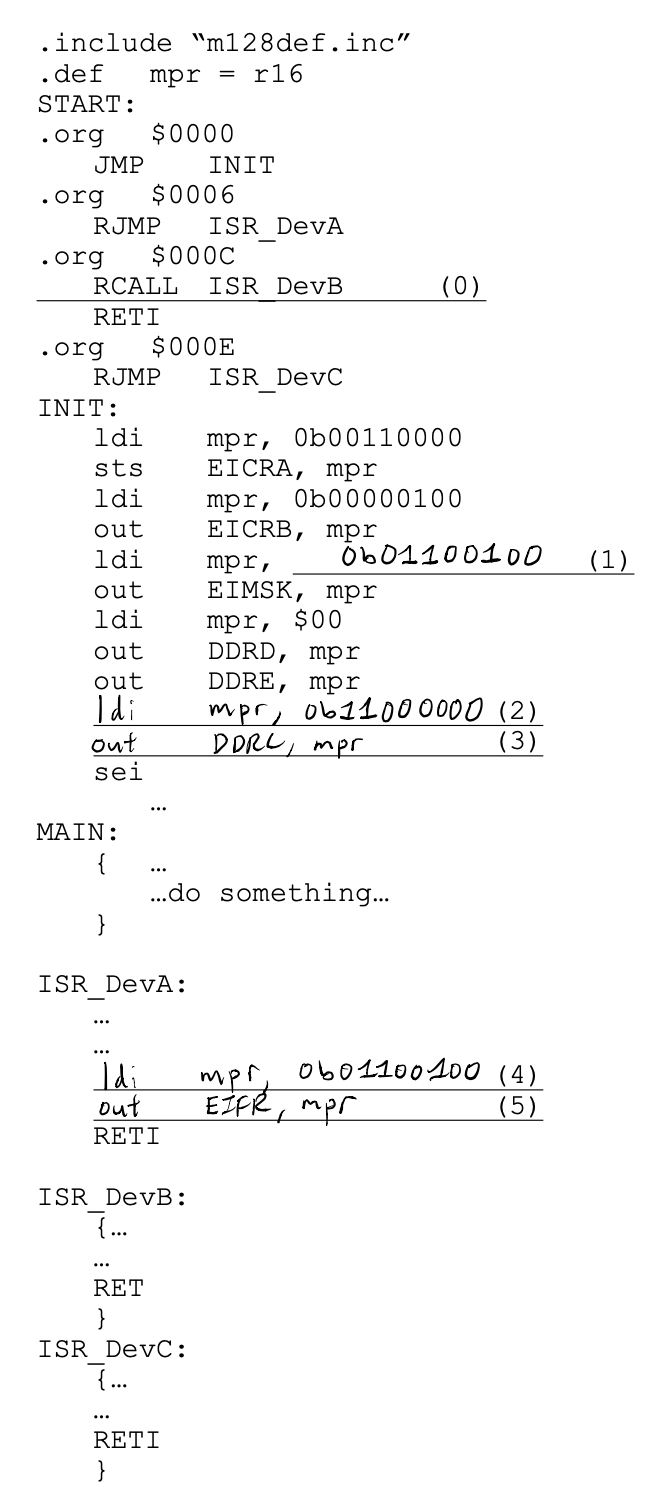
\includegraphics[width=0.35\linewidth]{p1.png}
    \caption{The completed code for problem 1.}
    \label{fig:p1}
  \end{figure}

  \begin{enumerate}
    \item The code places instructions for DevA, DevB, and DevC at interrupt vectors 0x0006, 0x000C, and 0x000E. Those vectors correspond to the external interrupt pins INT2, INT5, and INT6, respectively. To enable these interrupts, the corresponding bits in EIMSK must be set. INT2, INT5, and INT6 are enabled using bits 2, 5, and 6 of EIMSK, respectively. Therefore, the immediate value needed in line 1 is 0b01100100.

    \item DevC. The level or edge used to generate an interrupt is defined by the sense control bits in EICRA and EICRB one. For a low-level input, the bits ISCn1:ISCn0 must be 00. Out of the three interrupts used in the code, only INT6 has its sense control bits (ISC61:ISC60) set to 00, and INT6 is connected to DevC.

    \item To configure pins on Port C as outputs, the corresponding bits in the Port C Data Direction Register (DDRC) must be set. So for pins 7 and 6, bits 7 and 6 in that register should be set. So the value 0b11000000 is sent to DDRC:
      \begin{verbatim}
      ldi mpr, 0b11000000
      out DDRC, mpr
      \end{verbatim}

    \item To clear latched interrupts at the end of \texttt{ISR\_DevA}, we have to clear the corresponding bits in the External Interrupt Flag Register (EIFR). To clear a bit in that register, we write a 1 to the bit. There are three interrupts enabled, so three possible latched interrupts. To clear any latched interrupts on INT2, INT5, or INT6, we write 0b01100100 to EIFR:
      \begin{verbatim}
      ldi mpr, 0b01100100
      out EIFR, mpr
      \end{verbatim}

    \item No because there are conflicting instructions at the memory address 0x000E. Each interrupt vector has only two memory words (32 bits) of space. The \texttt{CALL} instruction itself is 32 bits long, so the \texttt{RETI} instruction would be stored at the address 0x000E. The problem is that the \texttt{RJMP ISR\_DevC} instruction is also placed at address 0x000E, so there is a conflict that should be caught by the assembler.

      Otherwise, if there were not a conflicting instruction at memory address 0x000E, this program would function correctly because after the \texttt{ISR\_DevB} function returns, it would execute the \texttt{RETI} instruction and return to where the program was executing before the interrupt, as expected.
  \end{enumerate}

\item The completed code for all parts of problem 2 is shown below in Figure \ref{fig:p2}. Explanations follow the figure.

  \begin{figure}[H]
    \centering
    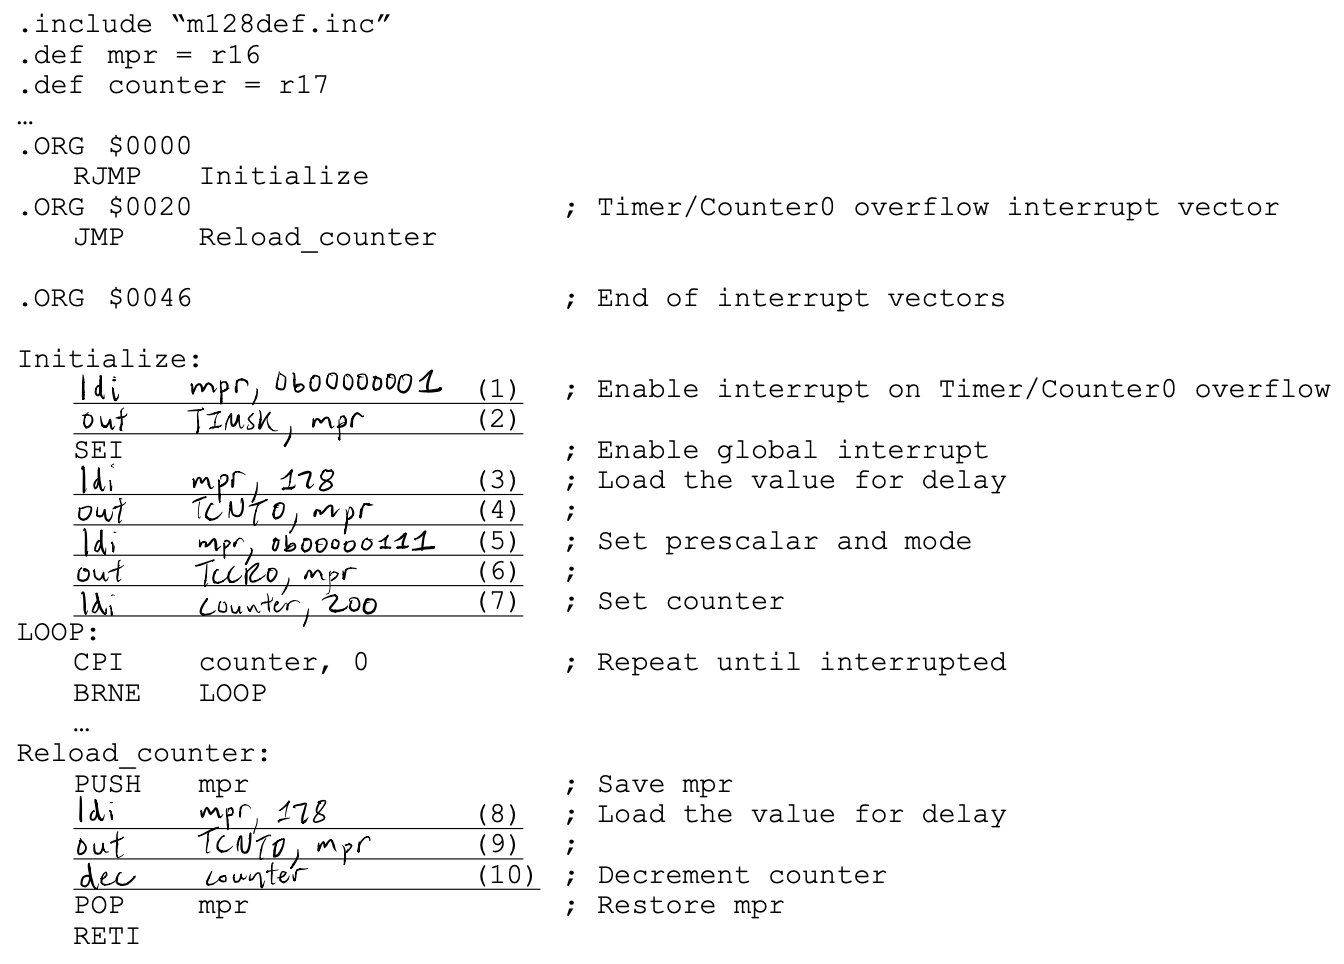
\includegraphics[width=0.5\linewidth]{p2.png}
    \caption{The completed code for problem 2.}
    \label{fig:p2}
  \end{figure}

  \begin{enumerate}
    \item To enable the Timer/Counter0 overflow interrupt, we have to set bit 0 of the Timer/Counter Interrupt Mask Register (TIMSK), which means loading the value 0b00000001 into TIMSK:
      \begin{verbatim}
      ldi mpr, 0b00000001
      out TIMSK, mpr
      \end{verbatim}

    \item To generate a delay of 5 milliseconds in normal mode, we need a value of $2^8 - \dfrac{16\text{ MHz}\cdot5\text{ ms}}{p}$, where $p$ is the prescaler. The only $p$ for which the value is positive is 1024, so the needed value is $2^8 - \dfrac{16\text{ MHz}\cdot5\text{ ms}}{1024} = 178$. So we load the value 178 into Timer/Counter0 Register (TCNT0):
      \begin{verbatim}
      ldi mpr, 178
      out TCNT0, mpr
      \end{verbatim}

    \item For a prescaler of 1024, the CS02:CS01:CS00 bits of the Timer/Counter0 Control Register (TCCR0) must be 111. And for normal mode, the WGM01:WGM00 bits are 00. I will assume that we OC0 should be disconnected here, so the COM01:COM00 bits are 00. Putting those bits together gives a value of 0b00000111 that should be sent to TCCR0:
      \begin{verbatim}
      ldi mpr, 0b00000111
      out TCCR0, mpr
      \end{verbatim}

    \item Each delay is 5 ms, so to create a 1 second delay, we need 200 5-millisecond delays. So the value 200 should be loaded into the counter:
      \begin{verbatim}
      ldi counter, 200
      \end{verbatim}

    \item To reload the value for delay (in order to create another 5 ms delay), we just load 178 into the Timer/Counter0 Register (TCNT0) again:
      \begin{verbatim}
      ldi mpr, 178
      out TCNT0, mpr
      \end{verbatim}

    \item To decrement \texttt{counter}, we just use the AVR \texttt{DEC} instruction:
      \begin{verbatim}
      dec counter
      \end{verbatim}
  \end{enumerate}

\item The completed code for all parts of problem 3 is shown below in Figure \ref{fig:p3}. Explanations follow the figure.

  \begin{figure}[H]
    \centering
    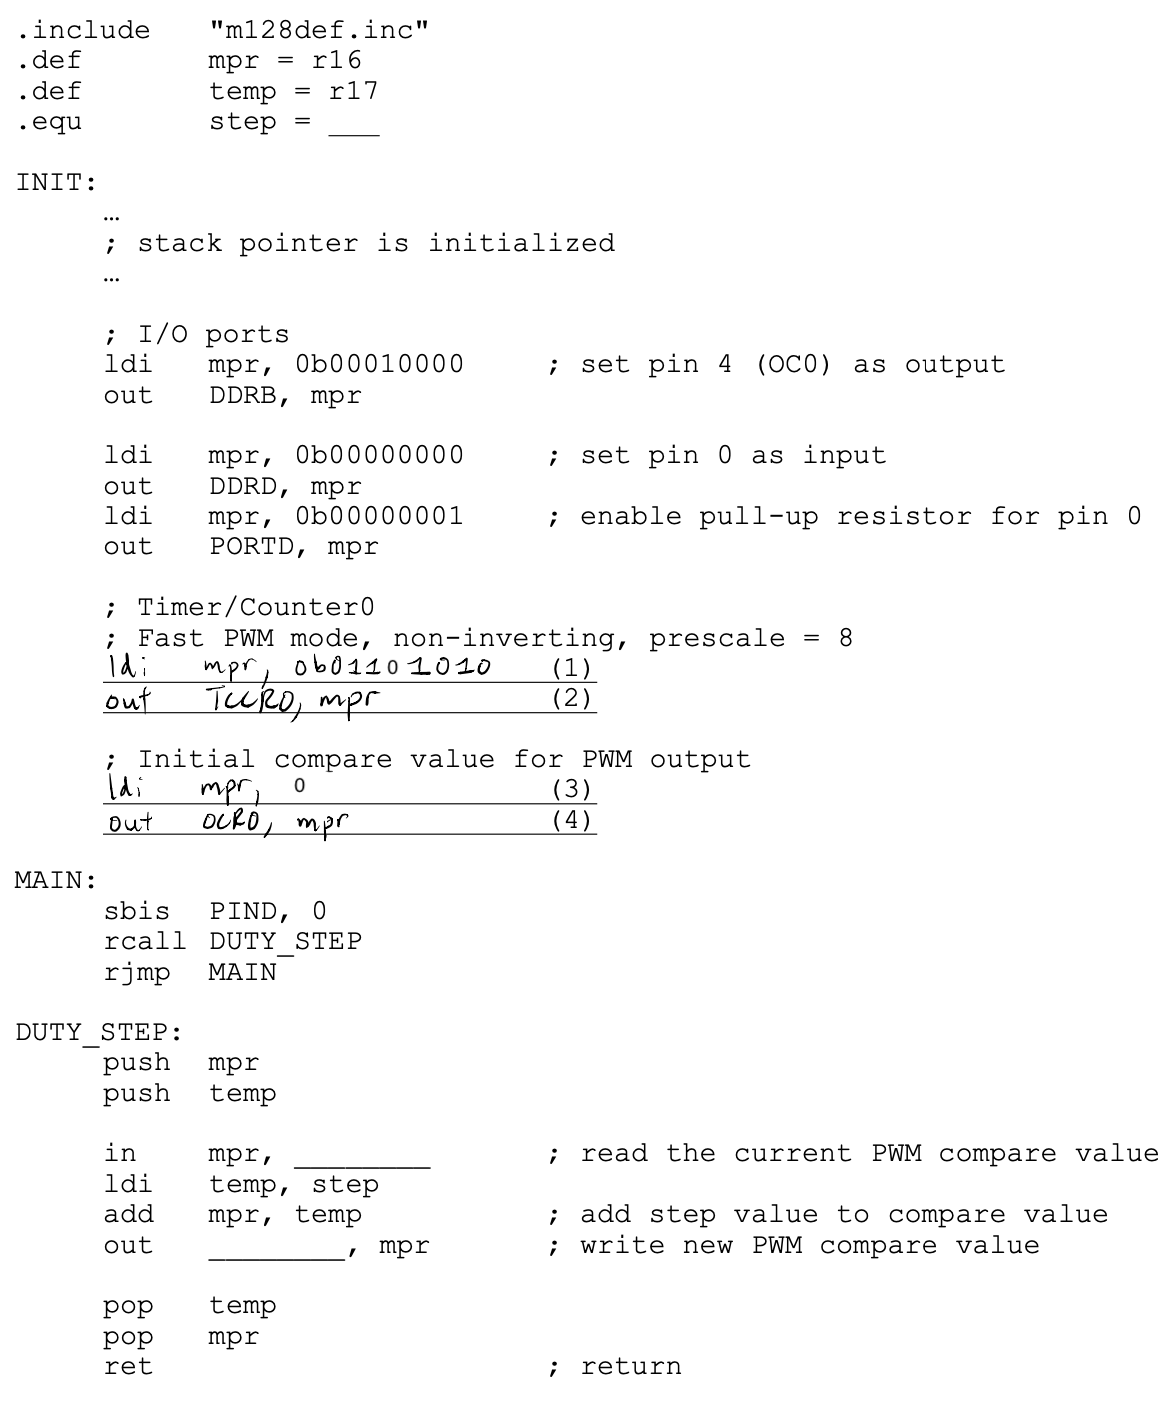
\includegraphics[width=0.43\linewidth]{p3.png}
    \caption{The completed code for problem 3.}
    \label{fig:p3}
  \end{figure}

  \begin{enumerate}
    \item To configure Timer/Counter0, we use the Timer/Counter0 Control Register (TCCR0). For Fast PWM mode, the WGM01:WGM00 bits are 11. For non-inverting mode, the COM01:COM00 bits are 10. And for a prescaler of 8, the CS02:CS01:CS00 bits are 010. Thus, we load the value 0b01111010 to TCCR0:
      \begin{verbatim}
      ldi mpr, 0b01101010
      out TCCR0, mpr
      \end{verbatim}

    \item For a given prescale value $p$, the frequency of the generated PWM signal is $f_{\text{PWM}} = \dfrac{clk_{\text{I/O}}}{p\cdot 256}$, so we have $f_{\text{PWM}} = \dfrac{16\text{ MHz}}{8\cdot 256} = 7812.5\text{ Hz}$.

    \item For a duty cycle of 0\%, we write the value 0 into Timer/Counter0's Output Compare Register (OCR0) because Timer/Counter0 is configured in non-inverting mode. That means the output OC0 is cleared on compare match and set at the bottom. With a duty cycle of 0\%, we never want OC0 to be set. Setting OCR0 to 0 means that OC0 will only be set when TCNT0 gets to 0, but that is also when OC0 gets cleared. That results in OC0 always being cleared, giving a 0\% duty cycle.
      \begin{verbatim}
      ldi mpr, 0
      out OCR0, mpr
      \end{verbatim}

    \item Since Timer/Counter0 is an 8-bit value, it can count up to a maximum of 255. Since $255/10 = 25.5$, we round up to 26. So to increase by duty cycle by 10\% each time the subroutine runs, the \texttt{step} variable should be 26.
  \end{enumerate}

\item To configure USART0 as an output, we set bit 1 of Port E's Data Direction Register (DDRE). To set the baud rate, we can calculate the value needed in the USART0 Baud Rate Register (UBRR0) using the equation $UBRR = \dfrac{f_{\text{OSC}}}{16BAUD} - 1 = \dfrac{16\text{ MHz}}{16\cdot 3000} - 1 = 332.33$. Since the UBRR value is a decimal, I will take the value 332, which gives a baud rate of 3003. In hex, 332 is 0x14C, so 0x01 will be loaded to UBRR0H, while 0x4C will be loaded to UBRR0L.

  Next, to enable the transmitter and the data register empty interrupt, we set the USART Data Register Empty Interrupt Enable (UDRIE0) and Transmitter Enable (TXEN0) bits of the USART0 Control and Status Register B (UCSR0B), giving a value of 0b00101000.

  Then, to set asynchronous mode and the frame format, we write to the USART0 Control and Status Register C (UCSR0C) and Register B (UCSR0B). For asynchronous mode, the UMSEL0 bit should be 0. For odd parity, the UPM01:UPM00 bits should be 11. For 1 stop bit, the USBS0 bit should be 0. And for 8 data bits, the UCSZ02:UCSZ01:UCSZ00 bits should be 011. Putting all those together gives a value of 0b00110110 for UCSR0C. The UCSZ02 bit is in UCSR0B, but its value is 0, so the value of UCSR0B remains 0b00101000.

  Finally, the global interrupt enable bit is set using the AVR \texttt{SEI} instruction. The full code is below:

  \begin{verbatim}
  .include "m128def.inc"
  .def mpr = r16
  .ORG $0000
    RJMP initUSART0
      ...
  .ORG $0026
    RJMP SendData
      ...
  .ORG $0046
  initUSART0:
    ...
    ...Your code goes here. The lines below provide hints as to what you should do...
    ; Configure USART0 (Port E, pin 1) as output
    ldi mpr, 0b00000010
    out DDRE, mpr
    ; Set baud rate to 3,000
    ldi mpr, $01
    out UBRR0H, mpr
    ldi mpr, $4C
    out UBRR0L, mpr
    ; Enable Transmitter and data register empty interrupt
    ldi mpr, 0b00101000
    sts UCSR0B, mpr
    ; Set asynchronous mode and frame format
    ldi mpr, 0b00110110
    sts UCSR0C, mpr
    ; Set the global interrupt enable bit
    sei
    ...
  Main:
    ld mpr, X+      ; Send first data
    out UDR0, mpr
  Loop:
    RJMP Loop

  SendData:
    ld mpr, X+      ; Send next data
    out UDR0, mpr
    reti
  \end{verbatim}

\end{enumerate}

\end{document}
